\section{Paleo-sea level compilations}

This is a list of paleo-sea level compilations, which served as the basis for this report. We acknowledge the hard work of the people compiling the data, as well as acknowledging those who collected the original data.

\subsection{North America}

\begin{itemize}
  \item Eastern Canada - \citet{VacchiEtal2018}
  \item Hudson Bay - \citet{SimonEtal2016}
  \item Greenland isolation basins - \citet{LongEtal2008}
  \item Eastern United States north of Georgia - \citet{EngelhartHorton2012}
\end{itemize}

For eastern Canada, the database by \citet{VacchiEtal2018} refered just to compilations (such as \citet{SimonEtal2016}) rather than the original sources. I have tried to track down the original sources as much as possible, but in some cases it was not possible. I made use of the compilations by \citet{SimonEtal2016},  \citet{GowanEtal2016} and an unpublished dataset by A.S. Dyke and T.S. James (some which was summarized in \citet{DykePeltier2000}) to track down references. Some were not listed in any of these compilations, so I had to track it down myself.

The MIS 3-5 data from the east coast of the United States was compiled by \citet{PicoEtal2017}.

Most of the data for Greenland was compiled by me, aside from the isolation basin dataset by \citet{LongEtal2008}. Though it did not contain a compilation of data, \citet{LecavalierEtal2014} listed references to a large number of studies that had sea level data. This was used to find the data used in this database. I also did a literature search for studies published after 2013.

\subsection{Europe}

\label{sec:Europe}

\begin{itemize}
  \item Baltic Sea - \citet{RosentauEtal2021}
  \item North Sea - \citet{VinkEtal2007}
\end{itemize}

The Baltic Sea sea level indicators are from \citep{RosentauEtal2021}. Note that some of the regions that they designated were really large with the gradient of the GIA, so I made smaller regions. This is why the regions in this report do not correspond to theirs in many places. Also note that Rosentau \emph{et al} chose to enter the radiocarbon dates for {\AA}ngermanland as pre-calibrated dates. I have not changed them.


The main compilation for the North Sea is by \citet{VinkEtal2007}. Though this predates the HOLSEA project, they use the indicative meaning concept and have a rigorous assessment of error, and is compatible with it. For Rotterdam, Netherlands, there is a HOLSEA compilation by \citet{HijmaCohen2019}. In Langeoog, there is a HOLSEA dataset by \citet{BungenstockEtal2021}. I have also included HOLSEA formatted data from Norderney \citep{SchederEtal2022}. Western Denmark does not a HOLSEA formatted compilation, so I added data compiled by \citet{GehrelsEtal2006} and \citet{JessenEtal2019}.


\subsection{Eurasian Arctic}

\begin{itemize}
  \item Northern Russia - \citet{BaranskayaEtal2018}
\end{itemize}

The compilation of sea level indicators for northern Russia comes from \citet{BaranskayaEtal2018}. Thank you to Alisa V. Baranskaya for sending the references (including translations from Russian) that were missing from the published compilation.

\subsection{Southeastern Asia}

\begin{itemize}
  \item Southeastern Asia (SEAMIS) - \citet{MannEtal2019}
\end{itemize}

The sea level indicators from southeastern Asia were compiled by \citet{MannEtal2019}. I corrected a number of errors, which are listed in the scratch datasets notes.

\subsection{Tropical Corals}

\begin{itemize}
  \item Tropical corals - \citet{HibbertEtal2016}
\end{itemize}

Corals from tropical regions were compiled by \citet{HibbertEtal2016}. In this report, I have taken indicators for Huon Peninsula, Vanuatu and French Polynesia from this database. An additional interpretation of the Huon Peninsula data comes from \citet{deGelderEtal2022}.

\subsection{Antarctica}

\begin{itemize}
  \item East Antarctica - \citet{IshiwaEtal2021}
  \item Antarctica - \citet{BriggsTarasov2013}
\end{itemize}

Currently, I have included two compilations from Antarctica. The compilation by \citet{IshiwaEtal2021} is focused on East Antarctica and includes MIS 3 data. The other is by \citet{BriggsTarasov2013}, and includes data from both West and East Antarctica for the Holocene. I also added a couple of sites not included in these compilations, including \citet{HjortEtal1997} and \citet{BraddockEtal2022}.

\subsection{Australia}

\begin{itemize}
  \item Australia - \citep{LewisEtal2013}
  \item New South Wales - \citet{SlossEtal2007}
  \item Queensland - \citet{LarcombeEtal1995}
  \item South Australia - \citet{BelperioEtal2002}
  \item Tasmania - \citet{Morrison2019}
\end{itemize}

The main compilation of Australia is from \citet{LewisEtal2013}. Thanks goes to Stephen E. Lewis, who kindly sent me the spreadsheets from this compilation and allowed me to include them in this database. This database was actually kind of a ``database of databases", which put together state databases, including New South Wales \citep{SlossEtal2007}, Queensland \citep{LarcombeEtal1995} and South Australia \citep{BelperioEtal2002}. Tasmania was not included in the Lewis paper because of a lack of studies. There is a compilation of Tasmania in \citet{Morrison2019}, which I have included. In addition, I have included the Great Barrier Reef data from \citet{YokoyamaEtal2018} and Bonaparte Gulf from \citet{YokoyamaEtal2000} and \citet{IshiwaEtal2019}.

\clearpage

\subsection{Data locations}

\begin{figure}[h]
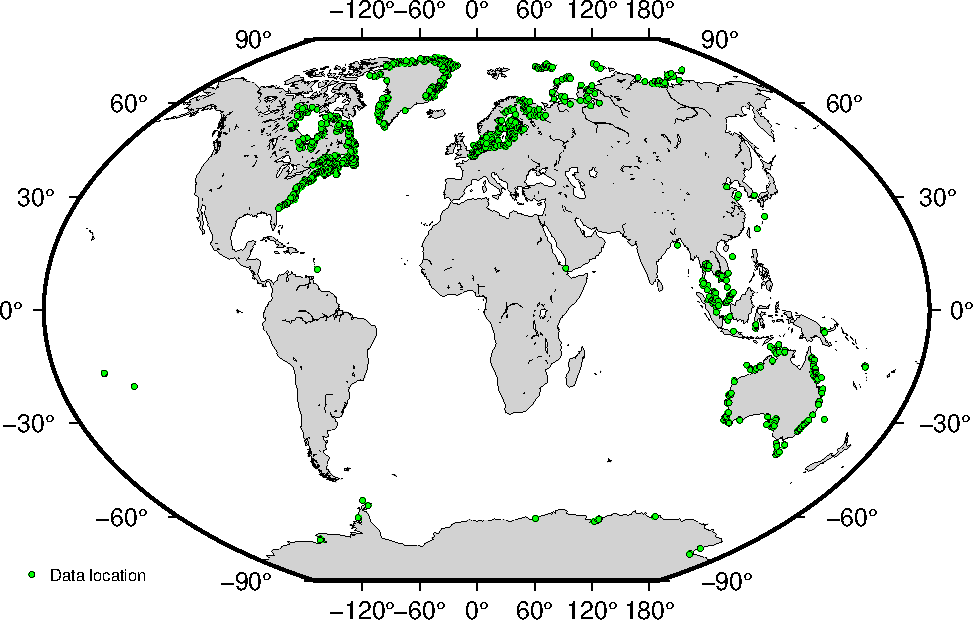
\includegraphics[width=\textwidth]{../GIS/data_map.pdf}
\caption{Map showing the location of data entered into the database.}
\label{fig:data_map}
\end{figure}

\clearpage
